\subsection{Balanço de potência}

\begin{figure}[H]
    \centering
    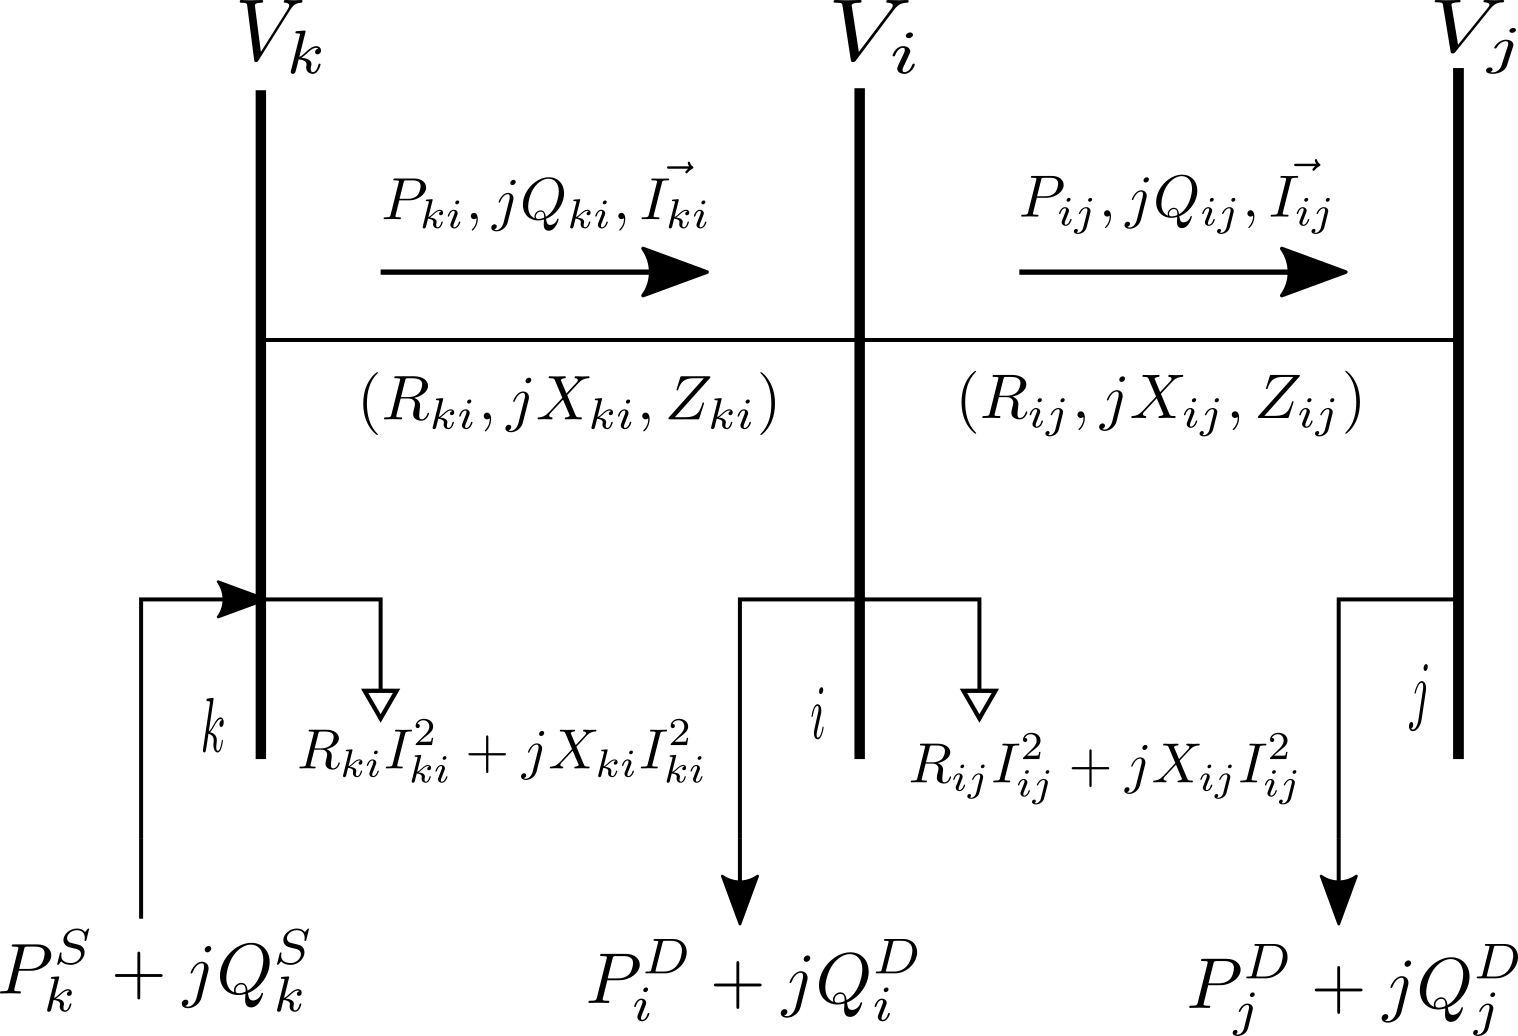
\includegraphics[width=0.6\textwidth]{3_Methodology/diagrama_nos.png}
    \caption{Exemplo de um diagrama de balanço de potência entre nós de um sistema de distribuição de energia elétrica}
    \label{fig:balanco_pot}
\end{figure}

A figura~\ref{fig:balanco_pot} representa a forma expandida da figura~\ref{fig:SDR}, para melhor compreensão do problema de balanço de potência, onde $m$ e $n$ representam um número qualquer de nós ligados ao nó $i$. 
Para isso considere que nos parâmetros e variáveis que representam um ramo, o primeiro subíndice representa o nó de partida e o segundo subíndice representa o nó de chegada (exemplo: $P_{12}$ se refere ao fluxo de potência ativa que vai do nó 1 para o nó 2).

Seja $P_{i}^{D}$ e $Q_{i}^{D}$ potência ativa e reativa demandada no nó i respectivamente e $P_{i}^{S}$ e $Q_{i}^{S}$ potência ativa e reativa gerada no nó $i$ respectivamente, têm-se que:

\begin{equation*}
    \sum_{ki\in\Omega_{l}}P_{ki} - \sum_{ij\in\Omega_{l}}(P_{ij} + R_{ij}I_{ij}^{2}) + P_{i}^{S} = P_{i}^{D}\quad\forall i \in\Omega_{b}
\end{equation*}

\begin{equation*}
    \sum_{ki\in\Omega_{l}}Q_{ki} - \sum_{ij\in\Omega_{l}}(Q_{ij} + X_{ij}I_{ij}^{2}) + Q_{i}^{S} = Q_{i}^{D}\quad\forall i \in\Omega_{b}
\end{equation*}

É possível mudar a variável \textit{k} pela variável \textit{j}, uma vez que ambas pertencem ao conjunto $\Omega_{l}$ e os somatórios envolvendo-as estão desconectados, além disso, pode-se realizar a troca de variável proposto em~\eqref{eq:change_variable}, obtendo assim as equações~\eqref{eq:fluxo_pot_ativa} e \eqref{eq:fluxo_pot_reativa}.
\begin{equation}
    \sum_{ji\in\Omega_{l}}P_{ji} - \sum_{ij\in\Omega_{l}}(P_{ij} + R_{ij}I_{ij}^{sqr}) + P_{i}^{S} = P_{i}^{D}\quad\forall i \in\Omega_{b}\label{eq:fluxo_pot_ativa}  
\end{equation}

\begin{equation}
    \sum_{ji\in\Omega_{l}}Q_{ji} - \sum_{ij\in\Omega_{l}}(Q_{ij} + X_{ij}I_{ij}^{sqr}) + Q_{i}^{S} = P_{i}^{D}\quad\forall i \in\Omega_{b}\label{eq:fluxo_pot_reativa}
\end{equation}

O sistema de equações não lineares em \eqref{eq:fluxo_pot_ativa} e \eqref{eq:fluxo_pot_reativa} representam a operação em regime permanente de uma rede elétrica radial e são frequentemente utilizados no método de varredura de fluxo de carga \cite{Shirmohammadi1988ANetworks} e \cite{Cespedes1990NewNetworks}.